\documentclass{beamer}
%
% Choose how your presentation looks.
%
% For more themes, color themes and font themes, see:
% http://deic.uab.es/~iblanes/beamer_gallery/index_by_theme.html
%
\mode<presentation>
{
  \usetheme{Singapore}      % or try Darmstadt, Madrid, Warsaw, ...
%   \usecolortheme{crane} % or try albatross, beaver, crane, ...
  \usefonttheme{default}  % or try serif, structurebold, ...
  \setbeamertemplate{navigation symbols}{}
  \setbeamertemplate{caption}[numbered]
} 

\addtobeamertemplate{navigation symbols}{}{%
    \usebeamerfont{footline}%
    \usebeamercolor[fg]{footline}%
    \hspace{1em}%
    \insertframenumber/\inserttotalframenumber
}

\usepackage[english]{babel}
\usepackage[utf8x]{inputenc}

\title[SISEC 2.0]{Signal Separation Evaluation Challenge\\2016 campaign and questions about the future}
\author{Antoine Liutkus, Inria\\ Fabian Stoeter, AudioLabs}
\date{22.2.2017}

\begin{document}

\begin{frame}
  \titlepage
\end{frame}

\begin{frame}{Outline}
 \tableofcontents
\end{frame}

\section{Introduction}

\begin{frame}{Before SiSEC}

There existed single task evaluation campaigns with, related to speech
signal:

\begin{itemize}

\item
  PASCAL Speech Separation Challenge I
\item
  PASCAL Speech Separation Challenge II
\item
  Lucas Parra's evaluation
\item
  Stereo Audio Source Separation Evaluation Campaign
\item
  MLSP'05 Data Analysis Competition
\item
  MLSP'06 Data Analysis Competition
\item
  MLSP'07 Data Analysis Competition
\end{itemize}

\end{frame}

\begin{frame}{The Signal Separation Evaluation Challenge}


\begin{itemize}
\item Combine various tasks and report during LVA/ICA. 
\item Roughly every 1.5 year: 2008, 2011, 2013, 2015
\item Each task is supervised by individual maintainer.
\item Targetted at all signal separation applications\\\textcolor{gray}{$\Rightarrow$ in practice mostly in audio}
\end{itemize}

\end{frame}

\section{Results SiSEC 2016}

\begin{frame}{SiSEC 2016}

\begin{itemize}

\item[UND]
  Underdetermined speech and music mixtures\\ \textcolor{gray}{1 new participant 2016} 
\item[BGN]
  Stereo mixtures of speech and real-world background noise\\ \textcolor{gray}{3 new participants 2016} 
\item[BIO]
  Separation of biomedical signals \textcolor{red}{new task}\\ \textcolor{gray}{2 participants 2016} 
\item[MUS]
  Professionally produced music recordings \textcolor{red}{new dataset}\\ \textcolor{gray}{16 new systems evaluated 2016} 
\end{itemize}

\end{frame}

\begin{frame}{SiSEC Impact}
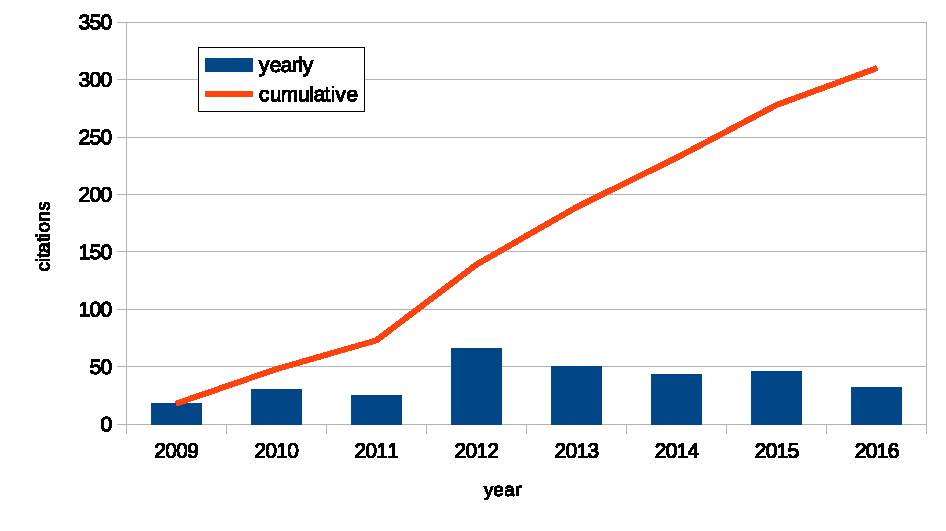
\includegraphics[width=\textwidth]{fig/SiSEC_impact-eps-converted-to.pdf}
\end{frame}

\begin{frame}{BGN: Stereo mixtures of speech and noise}
\centering
\includegraphics[width=0.6\textwidth]{fig/BGN-highlight.eps}
\begin{itemize}
\item Very different separation performance depending on metric. \\ \textcolor{gray}{$\Rightarrow$ Focus on speech quality ? Perceptual measurements\\$\Rightarrow$ Focus on application ? ASR performance: Chime challenge}
\end{itemize}
\end{frame}

\begin{frame}{BIO: Separation of biomedical signals}
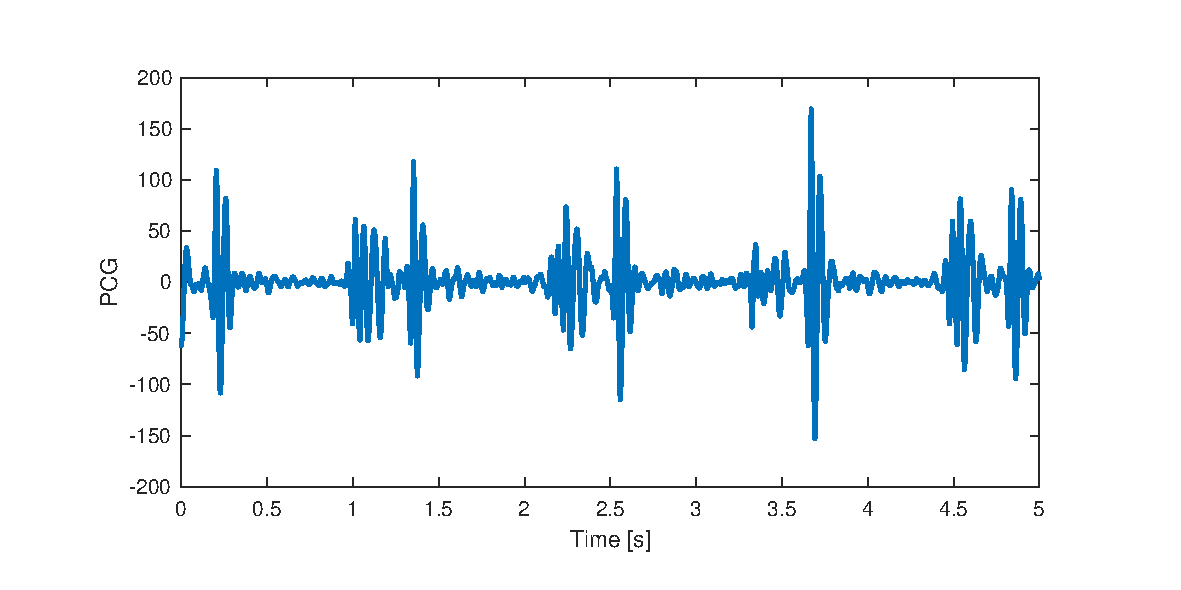
\includegraphics[width=\textwidth]{fig/BIO-PCG.pdf}
\begin{itemize}
\item Extract heart signal from raw acoustic recordings
\item Interferences from speech, cough, gastric noise, ...
\end{itemize}
\end{frame}

\begin{frame}{BIO: Separation of biomedical signals}
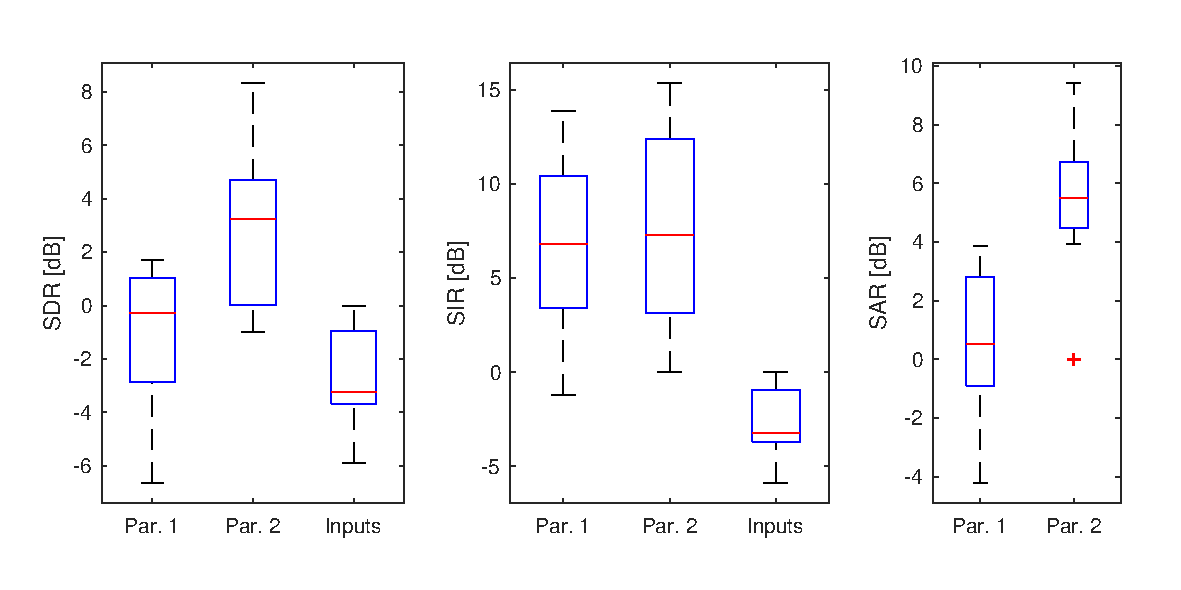
\includegraphics[width=\textwidth]{fig/BIO-results.pdf}
\begin{itemize}
\item Two methods based on empirical mode decompositions
\item Small dataset, some interest\\\textcolor{gray}{Develop evaluation of biomedical signal separation ?}
\end{itemize}

\end{frame}

\begin{frame}{MUS: Separation of music}
\begin{itemize}
\item 50 dev + 50 test \textcolor{red}{full-length, produced, stereo} tracks
\item Separate bass, drums, vocals, other
\item 23 methods evaluated + Ideal Binary Mask
\begin{center}
\vspace{0.5cm}vocals SDR
\end{center}
\end{itemize}
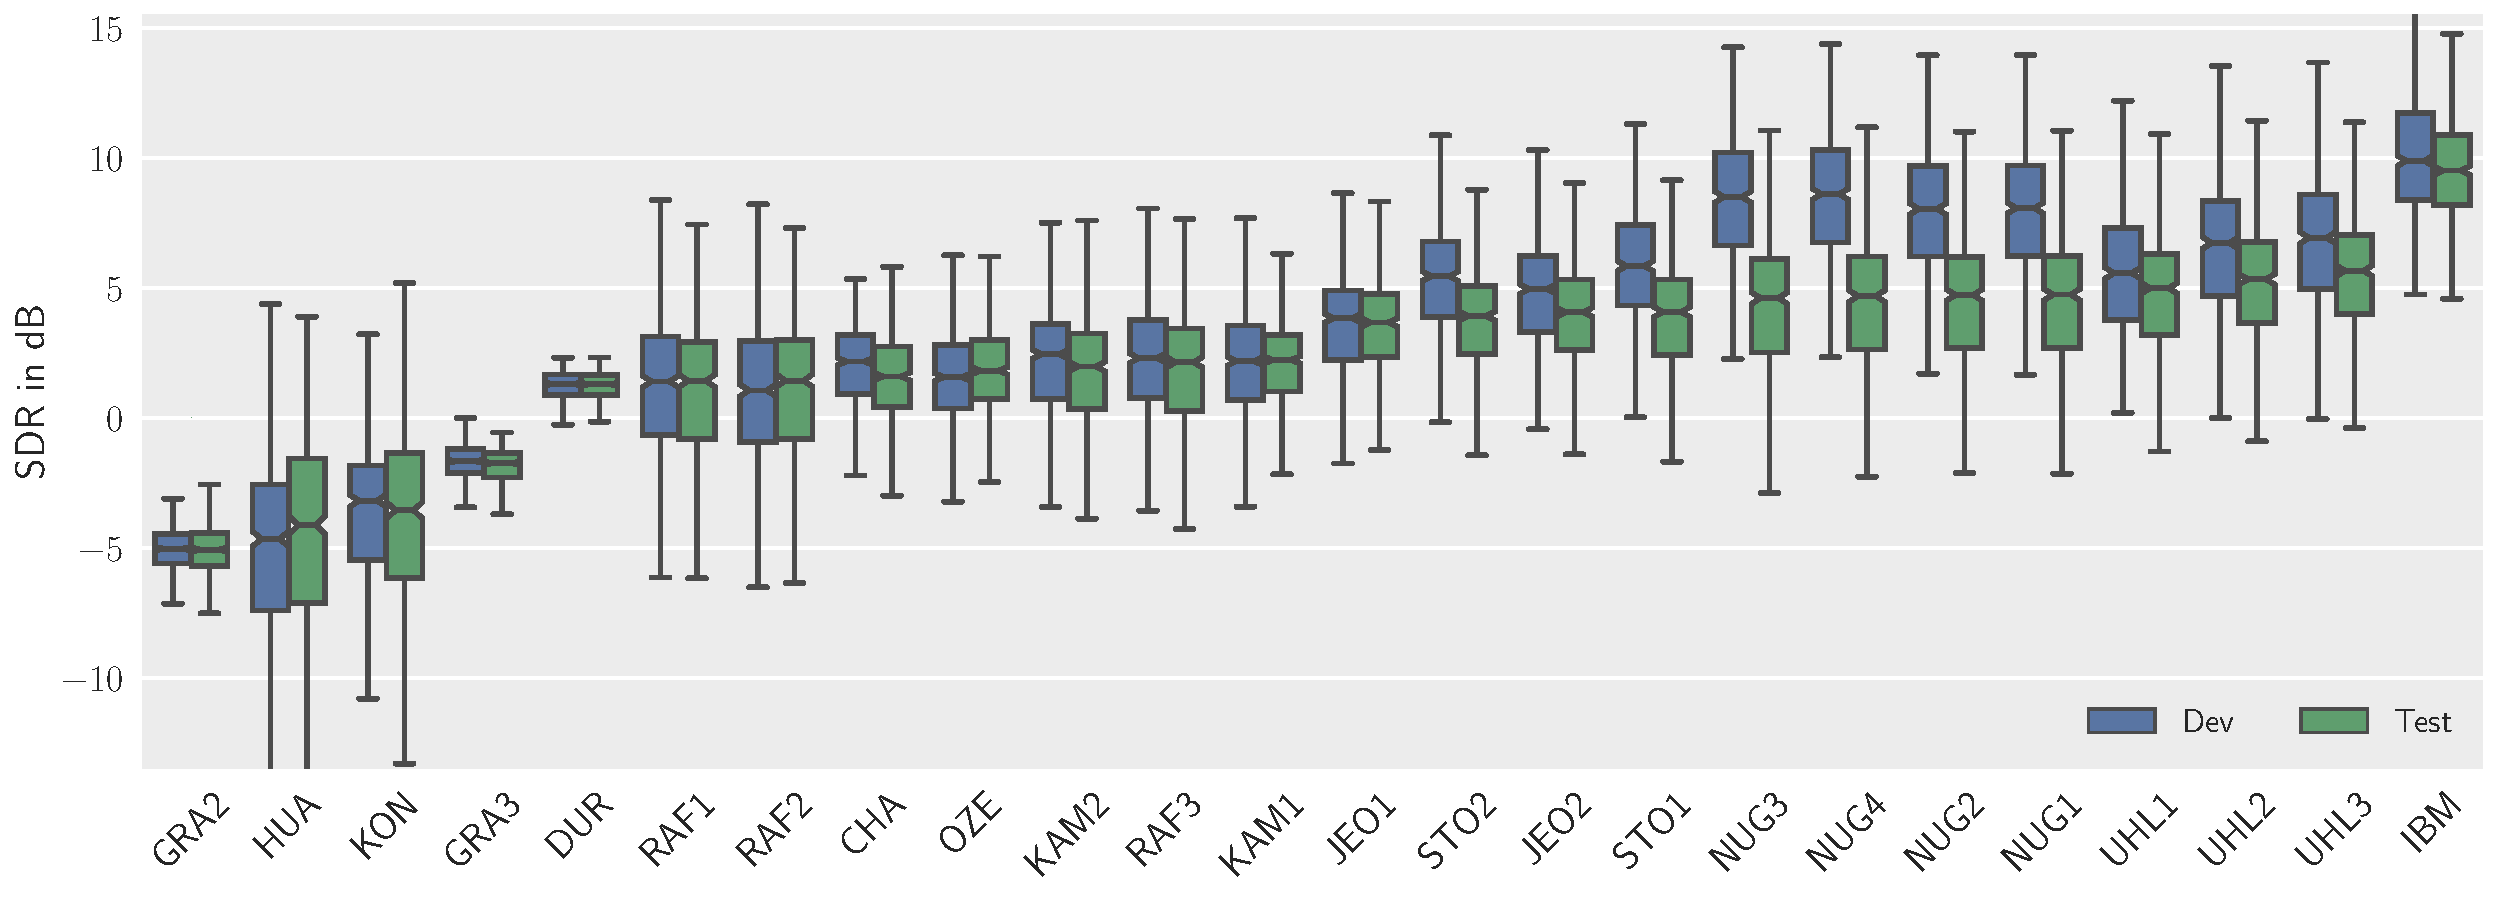
\includegraphics[width=\textwidth]{fig/MUS_SDR.pdf}
\end{frame}

\begin{frame}{MUS: Pair-wise comparisons}
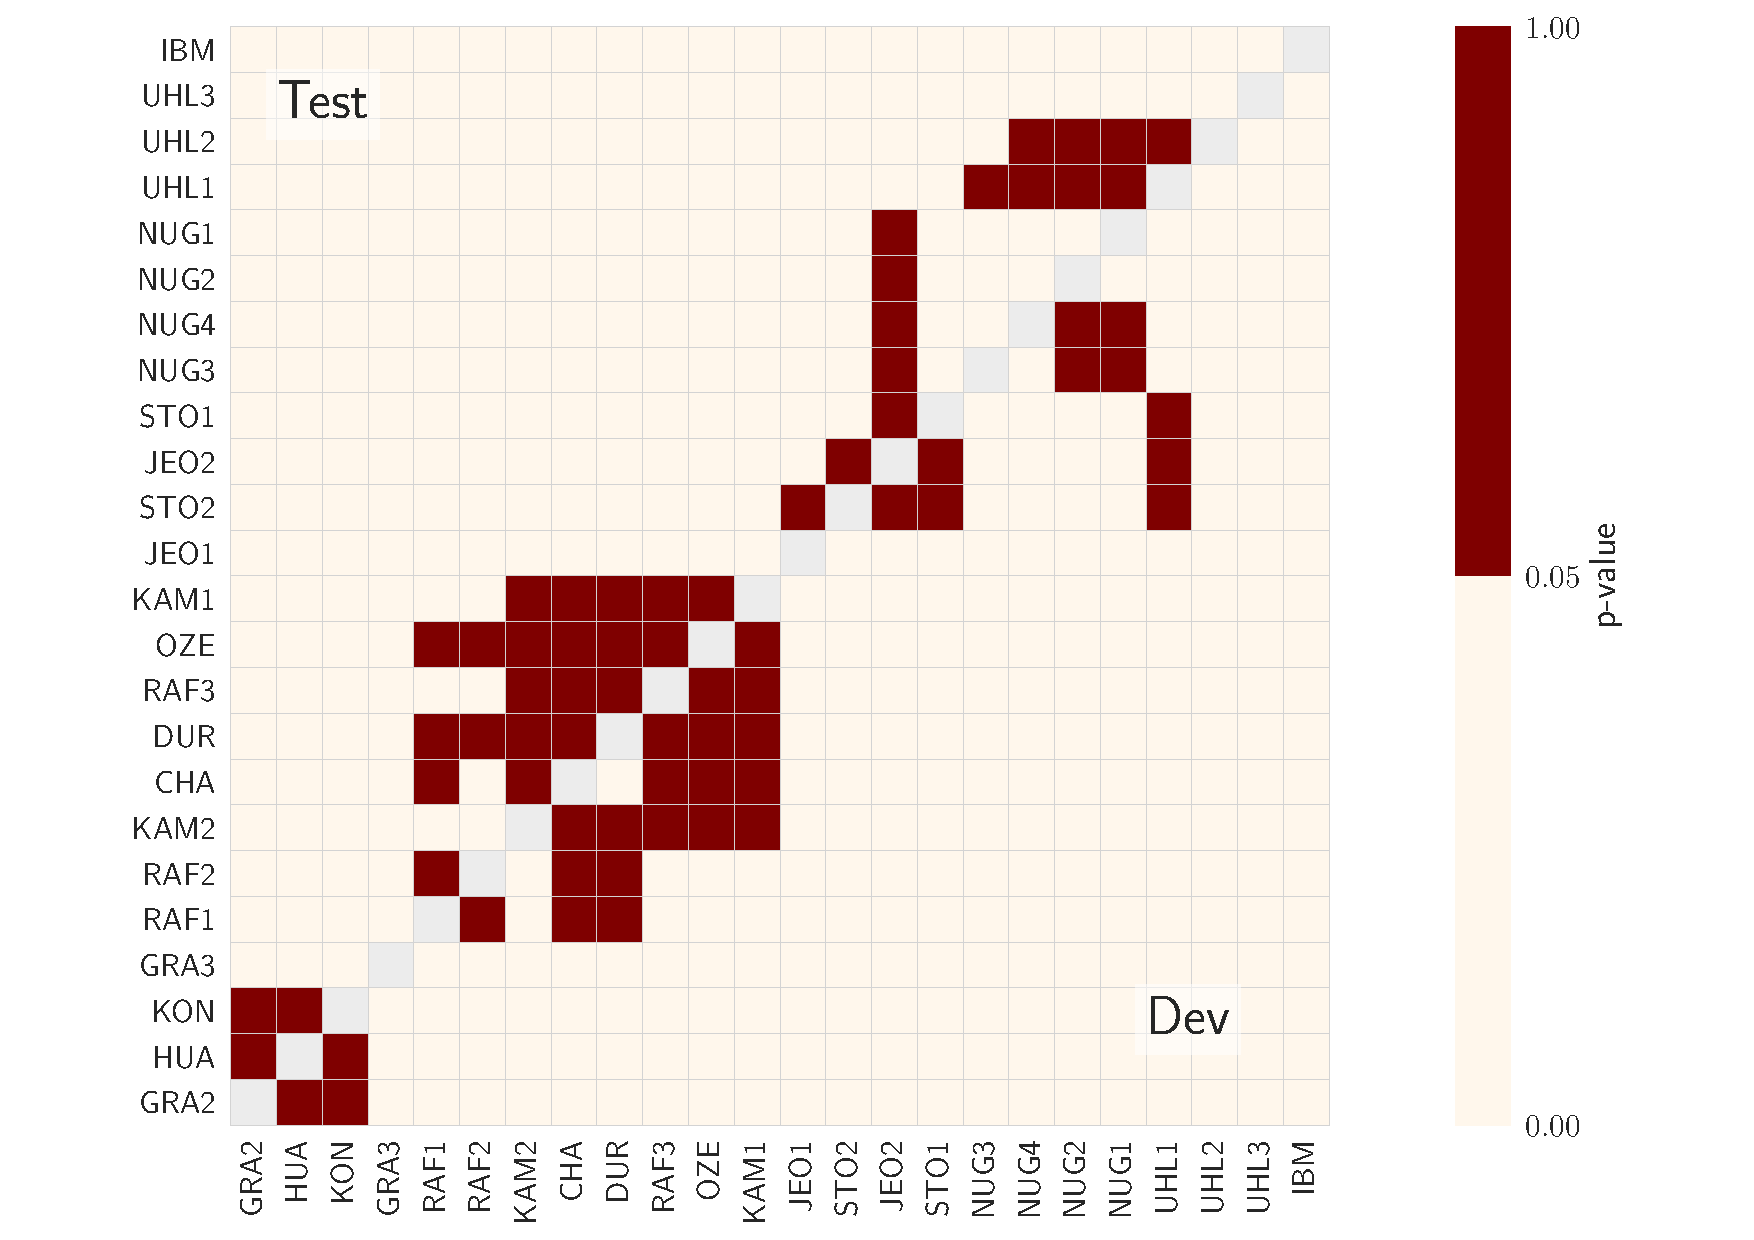
\includegraphics[width=\textwidth]{fig/wilcox_voc_sdr_slide.pdf}
\end{frame}

\begin{frame}{MUS: Vocals SDR}
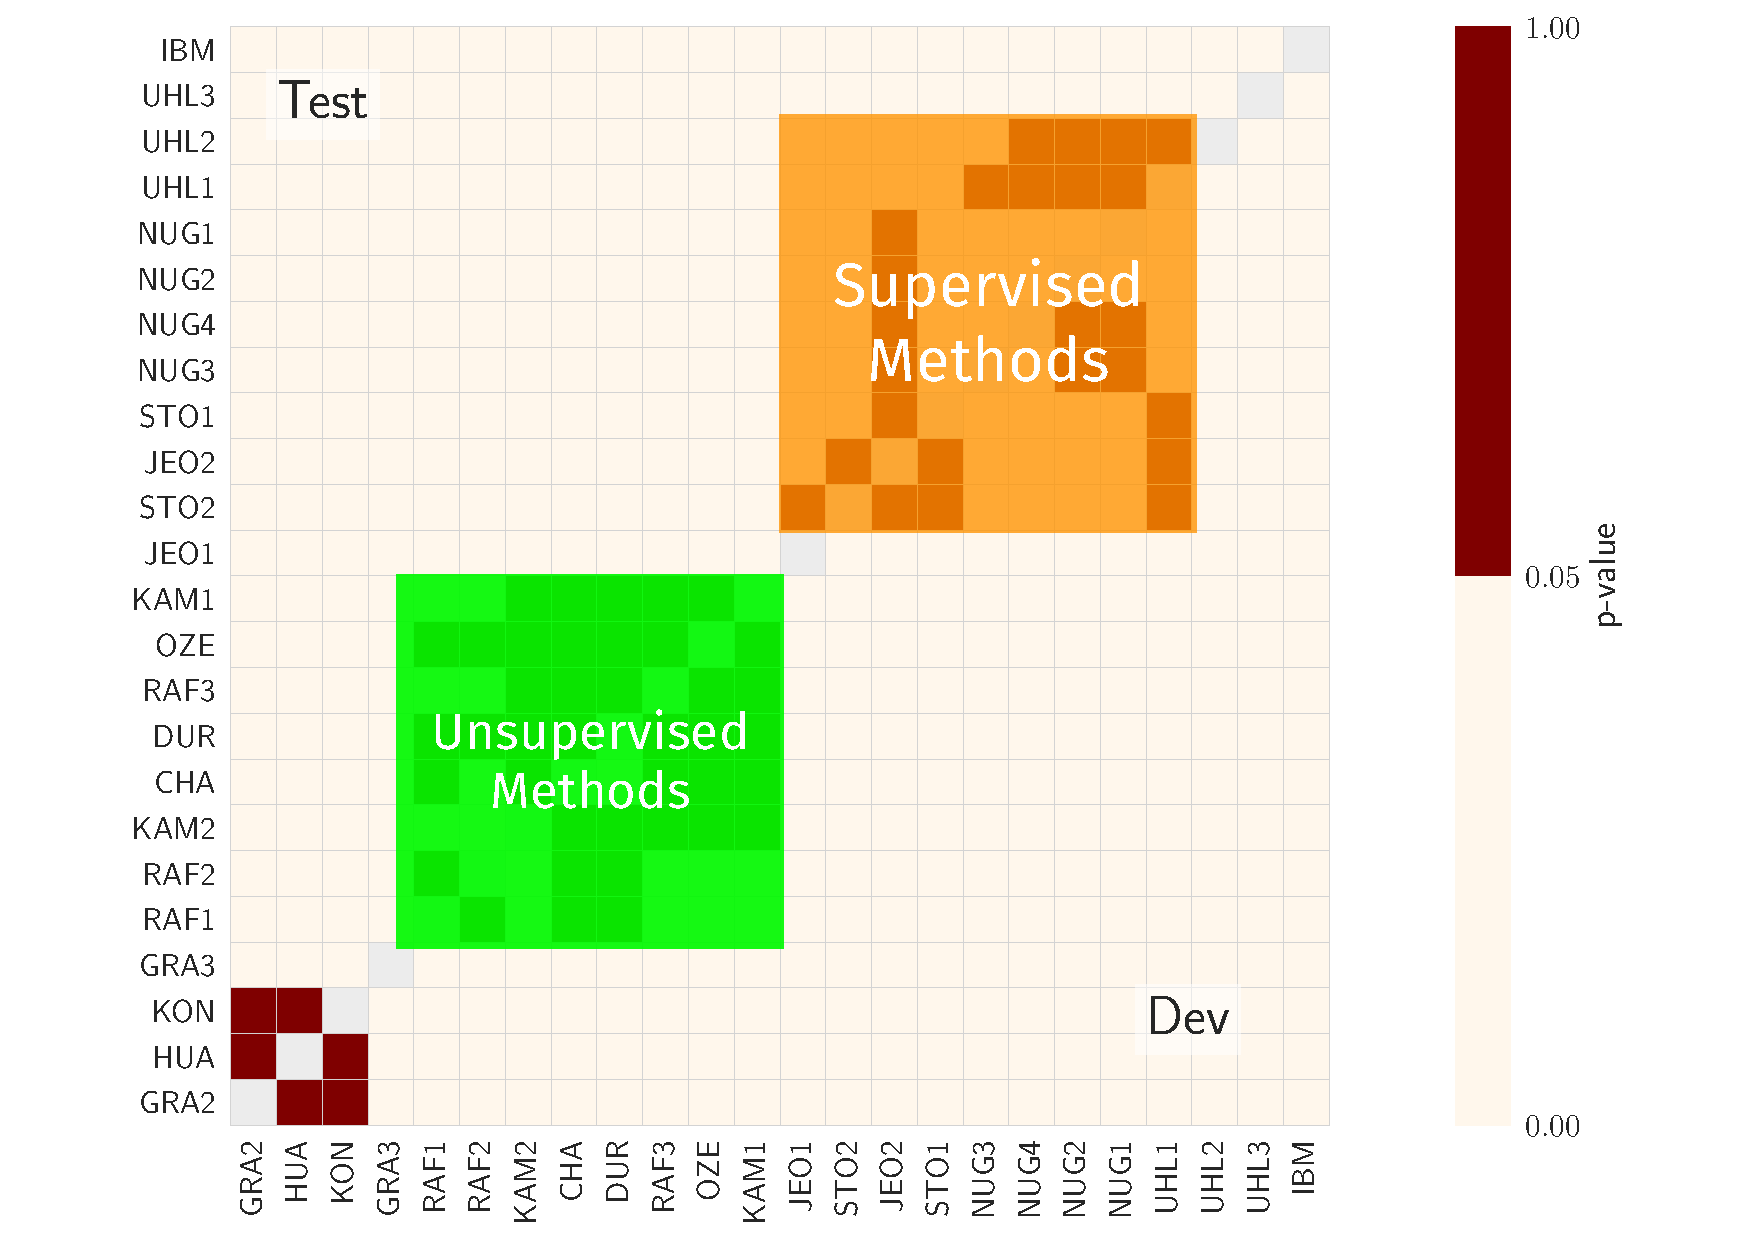
\includegraphics[width=\textwidth]{fig/wilcox_voc_sdr_slide_marked.pdf}
\end{frame}

\begin{frame}{DEMO: The 2016 MUS website}
\begin{center}
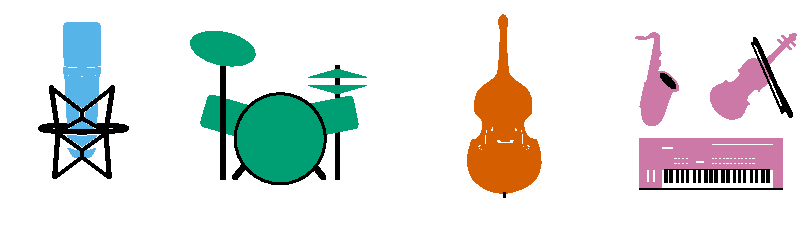
\includegraphics[width=\textwidth]{fig/mus-website.pdf}

\url{http://www.sisec17.audiolabs-erlangen.de}

\end{center}
\end{frame}

\section{Future of SiSEC}

\begin{frame}{Problems in SiSEC}

\begin{enumerate}
\def\labelenumi{\arabic{enumi}.}

\item
  Participation (except MUS).
\item
  Just data, no scripts (except MUS).
\item
  Visibility\\
  \textcolor{gray}{Once every 1.5 year is not enough\\LVA=Machine Learning scientists. Bridging the communities ?}
\item
  Only summary statistics, not actual separation results.
\item
  No baseline methods for simple comparison, sanity check.\\
  \textcolor{gray}{Provide minimum working examples?}
\end{enumerate}
\end{frame}

\begin{frame}
\textbf{How do others deal with these problems?}
\end{frame}

\begin{frame}{Industry: Kaggle}

\begin{itemize}
\item Platform for competitions on which
companies and researchers post their data and participants submit their results online. 

\item 3.500 competition submissions per day. 
\item Best submissions receive \$ (up to \$1M). 
\item Also used for academic challenges; e.g.:
\href{https://www.kaggle.com/c/mlsp-2013-birds}{MLSP 2013 Bird
Classification Challenge}
\end{itemize}

\begin{itemize}
\item \textcolor{gray}{Hosting only if organisers provide prizes in cash}
\item \textcolor{gray}{Evaluation limited to few metrics (mostly classification)}
\end{itemize}

\end{frame}

\begin{frame}{Academia: From MIREX to Open-MIC}

\begin{itemize}
\item MIR-Community is running a similar competition (MIREX) since 2005. 
\item Their problems:
\begin{itemize}
  \item
    high financial and labor costs (source code submissions)
  \item
    lack of data transparency
  \item
    lack of a strategy for obtaining and annotating new data
\end{itemize}
\item Proposal: Open-MIC\footnote{\href{https://github.com/cosmir/open-mic}{B. McFee, E. J. Humphrey, and J. Urbano. A Plan for Sustainable MIR Evaluation}}
  \begin{itemize}
  \item
    Distributed computation to reduce operating costs
  \item
    Freely distributable audio facilitates reproducibility
  \item
    Incremental evaluation, automatically collecting new annotation data
  \end{itemize}
\end{itemize}
\end{frame}

% \begin{frame}{What is it Open-MIC?}

% is an open-source server system that provides the
% following infrastructure:

% \begin{itemize}

% \item
%   Uploader: A collection of audio files, with potentially varying signal
%   parameters, are uploaded into the CAS.
% \item
%   Task Builder: Having creating a normalized, uniquely identified
%   collection, a number of annotation ``tasks'' are created.
% \item
%   Annotation: Tasks are served to a web-based annotation tool guided by
%   some backend logic, where users select and submit annotations.
% \item
%   Dataset Compiler: Based on the the state of the task collection, a
%   labeled ``training'' set (audio and annotation) and unlabeled ``test''
%   (audio only) set are exported from the CAS.
% \end{itemize}

% \begin{block}{}
% Open-MIC is ready in June and will be evaluated for one single task of
% instrument identification for next MIREX.
% \end{block}

% \end{frame}

\begin{frame}{Addressing the issues of SiSEC}

Differences to MIREX/Open-MIC

\begin{itemize}
	\item Signal processing problem instead of labeling problem
	\item SiSEC targets other applications, too (e.g. BIO).
    \item SiSEC already has open data and does not depend on annotations
\end{itemize}
\end{frame}

\begin{frame}{1. Participation}

\begin{itemize}
\item
SiSEC has to keep up with the scientific interests of the community\\
\textcolor{gray}{ICA became LVA in 2010. What about LVA Challenge ?\\
It should be easy to submit new tasks/data all the time.\\Can you provide data?} 
\item
Cosmetic improvements: website (see SiSEC MUS 2017).\\
\textcolor{gray}{Are there other ways to communicate you feel are appropriate}
\item Advertise to the machine (deep) learning community ?\\
\textcolor{gray}{easily get the data as MNIST digits ? }

\end{itemize}

\end{frame}

\begin{frame}[fragile]{2. Data and software}

\begin{itemize}
\item SiSEC data publicly available, but hard to host (MUS=14 Gb)\\
\textcolor{gray}{sustainable solution: help through torrent seeding or \$\$\$ ?}
\item easy to use subsets / toy data (equivalent to MNIST)\\
\textcolor{gray}{Legacy tasks ? subtasks ?}
\item Python DSDTOOLS for MUS. \\ \textcolor{gray}{extend it to other tasks ?}
\\ \textcolor{gray}{use github for all software tools (github.com/lva)?}
\end{itemize}
\end{frame}

% \begin{frame}{Next steps}

% \begin{itemize}
%   \item
%     Make \texttt{dsdtools} even easier to use with Deep Learning
%     libraries, so that feature extractors can be used to build Test and
%     Train Tensors
%       \item
%     We would propose \texttt{lvatools} which provide a unique
%     interface to all tasks. Easy way to download datasets, parse the
%     data. etc.
% \end{itemize}
% \end{frame}

\begin{frame}{Visibility (1/3)}
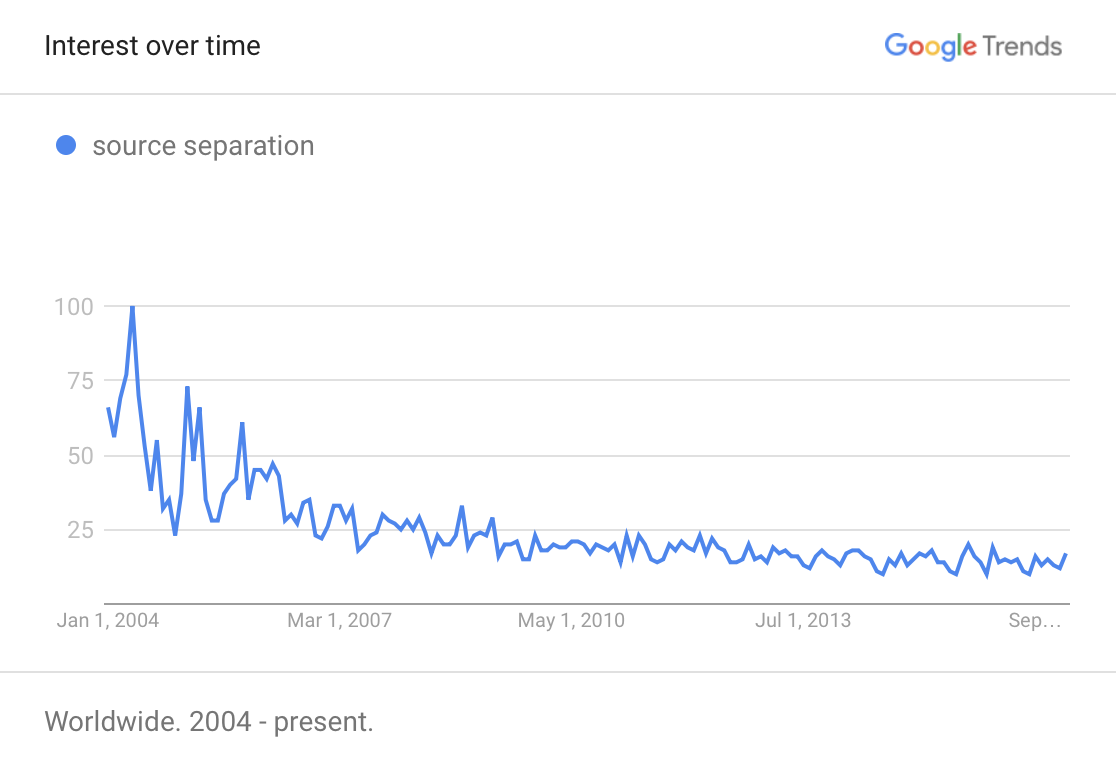
\includegraphics[width=\textwidth]{fig/source_separation.png}
\end{frame}

\begin{frame}{Visibility (2/3)}
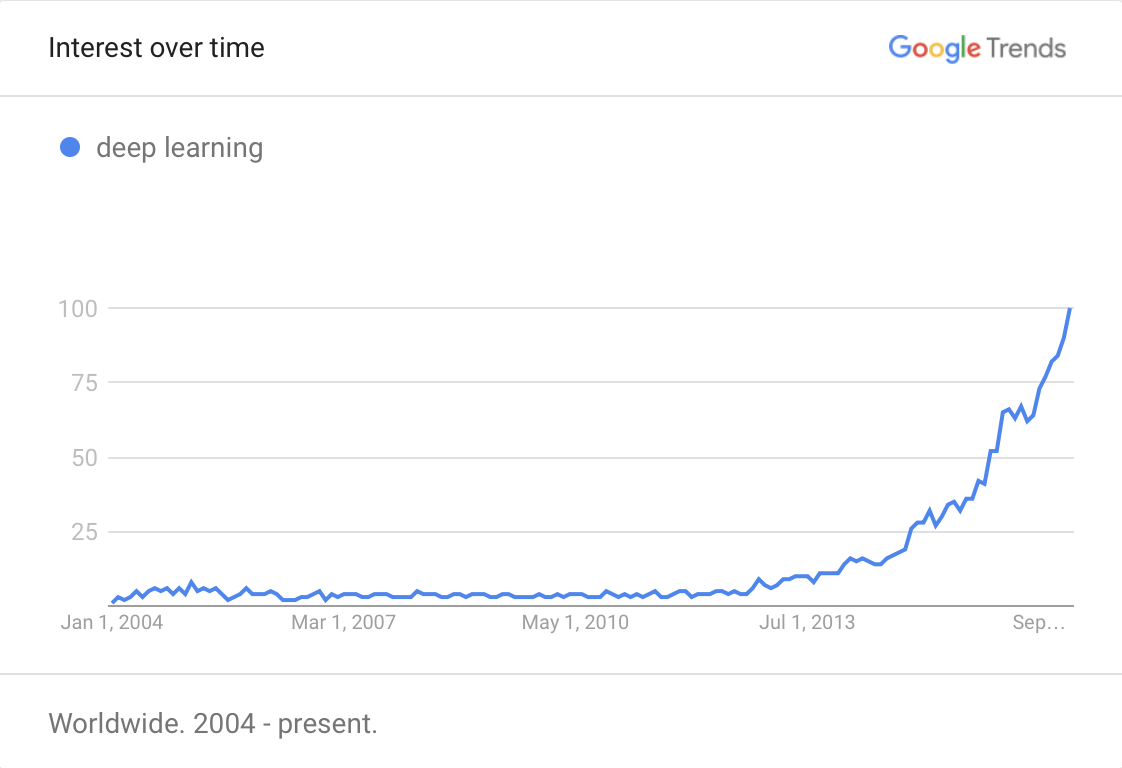
\includegraphics[width=\textwidth]{fig/deep_learning.png}
\end{frame}

\begin{frame}{Visibility (3/3)}
\begin{itemize}

\item Source separation is a difficult field to get into\\
\textcolor{gray}{But audio is seen as a great application !\\$\Rightarrow$ Provide toy data and minimum working examples.\\Can you provide baseline methods?}
\item The challenge should match the researchers' interest\\
\textcolor{gray}{Making it easy to propose a new task/data? How?}
\item Better exploit participation\\
\textcolor{gray}{Interactive web-report (see demo)\\
Sharing item-wise results and scores\\
Automatic results analysis: }\textcolor{red}{facilitating evaluation sections!}
\end{itemize}
\end{frame}

\begin{frame}{3. Automated evaluation}
\begin{enumerate}
\item Participants process test data themselves\\
\textcolor{gray}{lvatools should facilitate getting data and computing results\\software will be opensource (dsdtools is already)}
\item We compute the metrics\\
\textcolor{gray}{Automatic comparison with state of the art\\Figures generation\\Become state of the art!}
\item You can propose a metric (bsseval-like)\\
\textcolor{gray}{Compute on past evaluation results. }\\
\textcolor{red}{Interested in perceptual evaluation? Let's talk!}
\end{enumerate}

\vspace{0.5cm}What do you think of these? Do you have some experience?
\end{frame}

\begin{frame}{Sustainability and money!}


  \begin{itemize}

\item We want to host a lva server\\
\textcolor{gray}{thirdparty storage (i.e amazon) ?\\cloud computations?\\proprietary solutions?}\\
\item How can \textcolor{red}{you} contribute ?\\
\textcolor{gray}{Sponsor money ? National/international scientific projects?\\Provide sandboxes and computing power?}

\end{itemize}


\end{frame}

% \begin{frame}{5. Baseline methods are not easily accessible for simple
% comparison, sanity check.}

% To address this, we would propose to release open source baseline
% methods, under the SISEC organisation. These methods could be outdated
% but should be easy to use and run quickly.

% \begin{itemize}

% \item
%   Questions:

%   \begin{itemize}

%   \item
%     Can you provide baseline methods?
%   \end{itemize}
% \end{itemize}

% \end{frame}

\end{document}
